% Put labels, etc., on figures using PSTricks.
% Use dvips -E <file>.dvi -o <file>.eps to create encapsulated PostScript.
%
\documentclass[12pt]{article}
\usepackage{graphicx}
\usepackage{pstricks}
\pagestyle{empty}

\begin{document}
\rput(5,-5){
\rput(.1,-.1){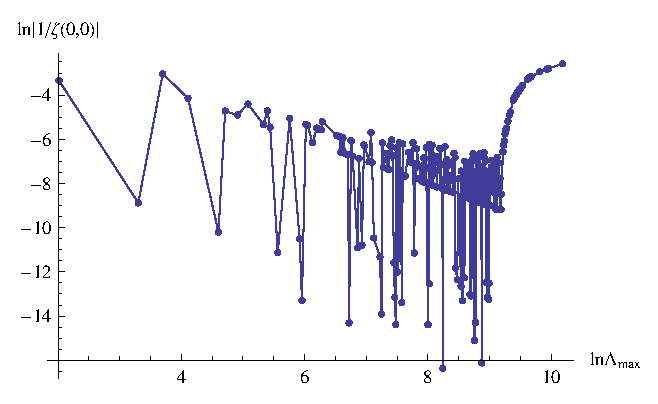
\includegraphics{../../thesis/figs_pst/skewUlamZeta.eps}}

\large

\psframe*[linecolor=white](-6.5,6)(-5.5,7)
\psframe*[linecolor=white](6,-6.5)(7.2,-5.5)

\rput(-2.9,2.8){$\Lambda_{max}=100$}
\rput(-0.5,1){$700$}
\rput(1.5,0){$3000$}
\rput(3.7,-1){$20000$}
\rput(6,-2.4){$10^5$}
\rput(7.8,-3.5){$5 \cdot 10^5$}
\rput(9,-4.5){$10^6$}
\psline[linewidth=1pt]{->}(-0.8,-1.9)(0.2,-0.6)\rput(-2,-2){$\Lambda_{max}=\infty$}


% Use grid command below to place objects at specified coordinates.
% \psgrid[subgriddiv=1,griddots=10](-9,-5.22)(8,8)
}
\end{document}
